%2multibyte Version: 5.50.0.2960 CodePage: 65001
% !TeX root = ./Slides_Lez_03_Valori_Attesi_Condizionati_verGPT_sh1.tex
% MQF - Lezione 3 - versione sintetica verGPT_sh1
% 18 slides, copertina inclusa. Scientific WorkPlace 5.5.
\documentclass[handout]{beamer}%
\usepackage{mathpazo}
\usepackage{multimedia}
\usepackage{amsmath}
\usepackage{amsfonts}
\usepackage{amssymb}
\usepackage{graphicx}
\setcounter{MaxMatrixCols}{30}
%TCIDATA{OutputFilter=latex2.dll}
%TCIDATA{Version=5.50.0.2960}
%TCIDATA{Codepage=65001}
%TCIDATA{CSTFile=beamer.cst}
%TCIDATA{<META NAME="DocumentShell" CONTENT="Other Documents\SW\Slides - Beamer">}
%BeginMSIPreambleData
\graphicspath{{../graphics/}}
\providecommand{\U}[1]{\protect\rule{.1in}{.1in}}
%EndMSIPreambleData
\newenvironment{stepenumerate}{\begin{enumerate}[<+->]}{\end{enumerate}}
\newenvironment{stepitemize}{\begin{itemize}[<+->]}{\end{itemize} }
\usetheme{Madrid}
\definecolor{light-blue}{rgb}{0.50,0.55,1.00}%
\setbeamertemplate{footline}
{
  \leavevmode%
  \hbox{%
    \begin{beamercolorbox}[wd=.20\paperwidth,ht=2.25ex,dp=1ex,center]
      {author in head/foot}%
      \usebeamerfont{author in head/foot}\insertshortauthor
    \end{beamercolorbox}%
    \begin{beamercolorbox}[wd=.69\paperwidth,ht=2.25ex,dp=1ex,center]
      {title in head/foot}%
      \usebeamerfont{title in head/foot}\insertshorttitle
    \end{beamercolorbox}%
    \begin{beamercolorbox}[wd=.11\paperwidth,ht=2.25ex,dp=1ex,right]
      {date in head/foot}%
      \usebeamerfont{date in head/foot}%
      \insertshortdate{}\hspace*{2em}%
      \insertframenumber{} / \inserttotalframenumber\hspace*{2ex}
    \end{beamercolorbox}%
  }%
  \vskip0pt%
}
% Macro ufficiali coerenti con MQF_Notazione.tex
\providecommand{\R}{\mathbb{R}}
\providecommand{\N}{\mathbb{N}}
\providecommand{\E}{\mathbb{E}}
\providecommand{\Prob}{\mathbb{P}}
\providecommand{\Q}{\mathbb{Q}}
\providecommand{\F}{\mathcal{F}}
\providecommand{\B}{\mathcal{B}}
\providecommand{\G}{\mathcal{G}}
\providecommand{\1}{\mathbf{1}}
\providecommand{\Var}{\operatorname{Var}}
\providecommand{\Cov}{\operatorname{Cov}}
\providecommand{\VaR}{\operatorname{VaR}}
\providecommand{\CVaR}{\operatorname{CVaR}}
\providecommand{\QTR}[2]{\csname #1\endcsname{#2}}
%BeginMSIPreambleData
\ifx\pdfoutput\relax\let\pdfoutput=\undefined\fi
\newcount\msipdfoutput
\ifx\pdfoutput\undefined\else
\ifcase\pdfoutput\else
\msipdfoutput=1
\ifx\paperwidth\undefined\else
\ifdim\paperheight=0pt\relax\else\pdfpageheight\paperheight\fi
\ifdim\paperwidth=0pt\relax\else\pdfpagewidth\paperwidth\fi
\fi\fi\fi
%EndMSIPreambleData

\title[Lez. 3 - Valori attesi condizionati e informazione]{Lezione 3 - Valori attesi condizionati e informazione}
\subtitle{Metodi Quantitativi per la Finanza}
\author[P. Falbo, C. Pelizzari]{{\LARGE Paolo Falbo, Cristian Pelizzari}}
\institute[]{{\large Dipartimento di Economia e Management}}
\date[]{}
\titlegraphic{

\includegraphics[height=1.25cm]{../graphics/MQF_logo.png}\hspace{0.8cm}%

\includegraphics[height=1.25cm]{../graphics/logo-Unibs-esteso.png}
}
\begin{document}
\maketitle

\section{Apertura e condizionamento a un evento}
%*********************************************
\subsection{Perch\`{e} condizionare?}
%TCIMACRO{\TeXButton{BeginFrame}{\begin{frame}}}%
%BeginExpansion
\begin{frame}%
%EndExpansion
\QTR{frametitle}{Perch\`{e} condizionare?}
%TCIMACRO{\TeXButton{Transparency}{\setbeamercovered{transparent=20}}}%
%BeginExpansion
\setbeamercovered{transparent=20}%
%EndExpansion

\begin{center}
{\Large Come cambia la valutazione di un payoff quando arriva nuova informazione?}
\end{center}
\medskip
Sia $H$ un payoff futuro, non ancora conosciuto.
\begin{itemize}
\item \textbf{Prima del segnale}: la valutazione \`{e} la media $\E[H]$.
\item \textbf{Dopo un segnale}: osserviamo un evento $A$ e rivediamo la media $\E[H\mid A]$.
\item Il payoff $H$ \textbf{non cambia}: cambia la distribuzione degli scenari
compatibili con l'informazione acquisita.
\end{itemize}
\medskip
\begin{center}
\textcolor{light-blue}{Il condizionamento traduce un'informazione osservata in una valutazione aggiornata.}
\end{center}

%TCIMACRO{\TeXButton{EndFrame}{\end{frame}}}%
%BeginExpansion
\end{frame}%
%EndExpansion
%*********************************************
\subsection{Il valore atteso condizionato a un evento}
%TCIMACRO{\TeXButton{BeginFrame}{\begin{frame}}}%
%BeginExpansion
\begin{frame}%
%EndExpansion
\QTR{frametitle}{Il valore atteso condizionato a un evento}
%TCIMACRO{\TeXButton{Transparency}{\setbeamercovered{transparent=20}}}%
%BeginExpansion
\setbeamercovered{transparent=20}%
%EndExpansion

\textbf{Ipotesi.} $X$ \`{e} integrabile, $A\in\F$ e $\Prob(A)>0$.
\medskip
\textbf{Definizione.} Il valore atteso di $X$ dopo aver osservato $A$ \`{e}
\[
\boxed{\E[X\mid A]=\frac{\E[X\1_A]}{\Prob(A)}.}
\]
Nel caso discreto, se $X$ assume valori $x_j$,
\[
\E[X\mid A]=\sum_j x_j\Prob(X=x_j\mid A).
\]
\begin{itemize}
\item La condizione $A$ seleziona gli scenari ancora possibili.
\item Le probabilit\`{a} condizionate sono i nuovi pesi della media.
\end{itemize}
\begin{center}
\textcolor{light-blue}{$\E[X\mid A]$ \`{e} un \textbf{numero}: l'evento osservato \`{e} gi\`{a} specificato.}
\end{center}

%TCIMACRO{\TeXButton{EndFrame}{\end{frame}}}%
%BeginExpansion
\end{frame}%
%EndExpansion

\section{Partizioni e sigma-algebre}
%*********************************************
\subsection{L'informazione come partizione di $\Omega$}
%TCIMACRO{\TeXButton{BeginFrame}{\begin{frame}}}%
%BeginExpansion
\begin{frame}%
%EndExpansion
\QTR{frametitle}{L'informazione come partizione di $\Omega$}
%TCIMACRO{\TeXButton{Transparency}{\setbeamercovered{transparent=20}}}%
%BeginExpansion
\setbeamercovered{transparent=20}%
%EndExpansion

\begin{center}
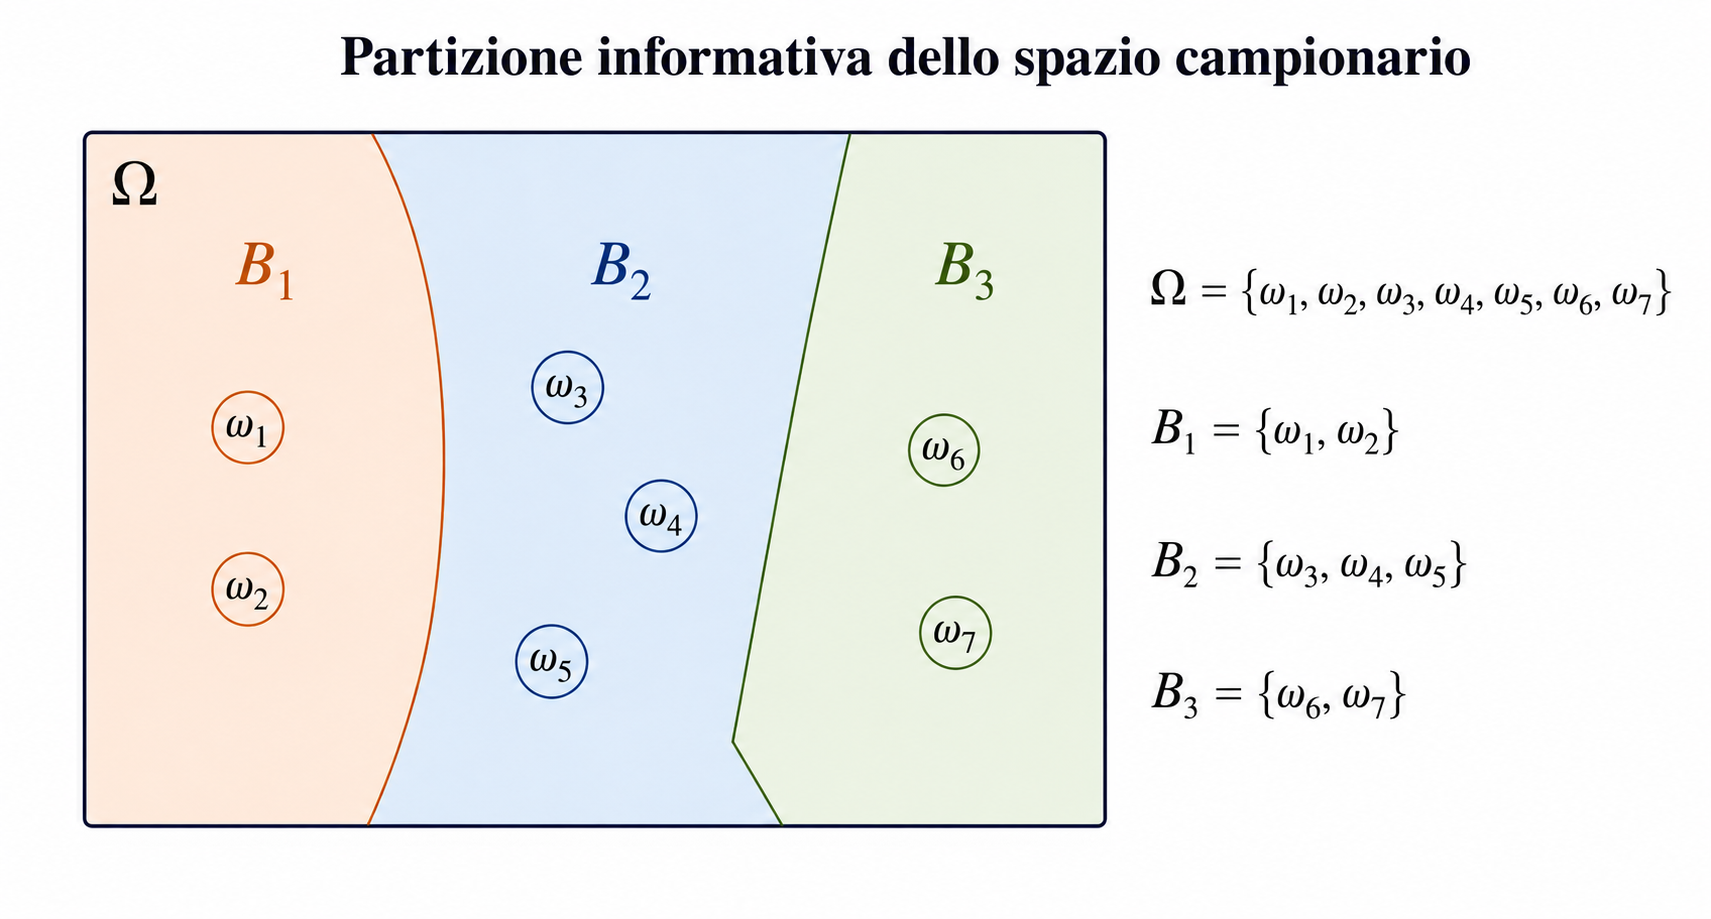
\includegraphics[width=0.74\textwidth,height=0.51\textheight,keepaspectratio]{Cap03_Figura_3_1.png}
\end{center}
\vspace{-2mm}
\[
\begin{aligned}
B_1&=\{\omega_1,\omega_2\},\\
B_2&=\{\omega_3,\omega_4,\omega_5\},\quad
B_3=\{\omega_6,\omega_7\}.
\end{aligned}
\]
\begin{center}
\textcolor{light-blue}{Il segnale rivela il blocco $B_i$, non necessariamente lo scenario $\omega$ dentro il blocco.}
\end{center}

%TCIMACRO{\TeXButton{EndFrame}{\end{frame}}}%
%BeginExpansion
\end{frame}%
%EndExpansion
%*********************************************
\subsection{La sigma-algebra generata dalla partizione}
%TCIMACRO{\TeXButton{BeginFrame}{\begin{frame}}}%
%BeginExpansion
\begin{frame}%
%EndExpansion
\QTR{frametitle}{La sigma-algebra generata dalla partizione}
%TCIMACRO{\TeXButton{Transparency}{\setbeamercovered{transparent=20}}}%
%BeginExpansion
\setbeamercovered{transparent=20}%
%EndExpansion

\begin{center}
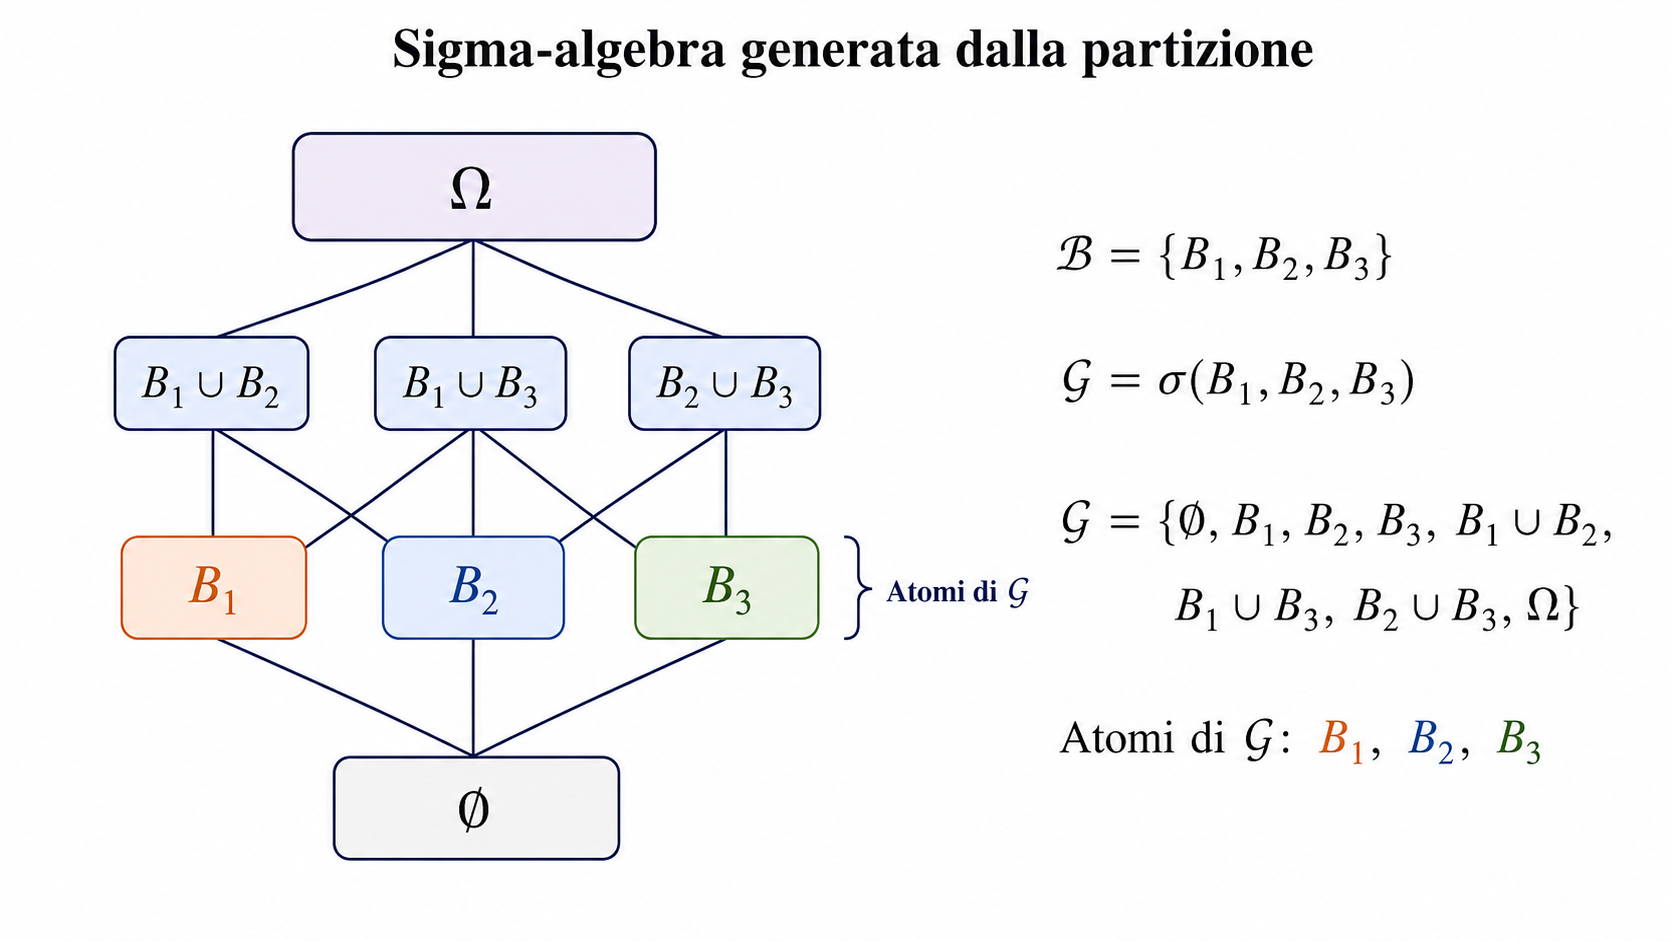
\includegraphics[width=0.75\textwidth,height=0.46\textheight,keepaspectratio]{Cap03_Figura_3_2.png}
\end{center}
\vspace{-1mm}
\[
\G=\sigma(B_1,B_2,B_3).
\]
\begin{itemize}
\item Gli \textbf{atomi} di $\G$ sono $B_1,B_2,B_3$.
\item Gli \textbf{eventi osservabili} sono le loro unioni (otto eventi, compresi $\varnothing$ e $\Omega$).
\end{itemize}

%TCIMACRO{\TeXButton{EndFrame}{\end{frame}}}%
%BeginExpansion
\end{frame}%
%EndExpansion

\section{Esempio con sette esiti}
%*********************************************
\subsection{Sette scenari: dal payoff alle medie locali}
%TCIMACRO{\TeXButton{BeginFrame}{\begin{frame}}}%
%BeginExpansion
\begin{frame}%
%EndExpansion
\QTR{frametitle}{Sette scenari: dal payoff alle medie locali}
%TCIMACRO{\TeXButton{Transparency}{\setbeamercovered{transparent=20}}}%
%BeginExpansion
\setbeamercovered{transparent=20}%
%EndExpansion

\small
\textbf{Dati.} Un payoff $H$ assume i valori seguenti nei sette scenari:
\medskip
\begin{center}
\begin{tabular}{c|cc|l}
Atomo & $\omega$ & $\Prob(\{\omega\})$ & $H(\omega)$ \\
\hline
$B_1$ & $\omega_1,\omega_2$ & $0.10,\ 0.15$ & $130,\ 110$ \\
$B_2$ & $\omega_3,\omega_4,\omega_5$ & $0.15,\ 0.20,\ 0.10$ & $100,\ 90,\ 80$ \\
$B_3$ & $\omega_6,\omega_7$ & $0.18,\ 0.12$ & $70,\ 50$
\end{tabular}
\end{center}
\medskip
\textbf{Calcolo.} Le medie sui blocchi sono
\[
\begin{aligned}
\E[H\mid B_1]&=\frac{0.10\cdot130+0.15\cdot110}{0.25}=118,\\
\E[H\mid B_2]&=\frac{0.15\cdot100+0.20\cdot90+0.10\cdot80}{0.45}=91.111\ldots,\\
\E[H\mid B_3]&=\frac{0.18\cdot70+0.12\cdot50}{0.30}=62.
\end{aligned}
\]

%TCIMACRO{\TeXButton{EndFrame}{\end{frame}}}%
%BeginExpansion
\end{frame}%
%EndExpansion
%*********************************************
\subsection{Dalle medie locali a una variabile casuale}
%TCIMACRO{\TeXButton{BeginFrame}{\begin{frame}}}%
%BeginExpansion
\begin{frame}%
%EndExpansion
\QTR{frametitle}{Dalle medie locali a una variabile casuale}
%TCIMACRO{\TeXButton{Transparency}{\setbeamercovered{transparent=20}}}%
%BeginExpansion
\setbeamercovered{transparent=20}%
%EndExpansion

\textbf{Costruzione.} L'informazione disponibile identifica un blocco
$B_i$, ma prima di osservarlo non sappiamo quale si realizzer\`{a}.
\medskip
\[
\boxed{Z=\E[H\mid\G]
=118\,\1_{B_1}+91.111\ldots\,\1_{B_2}+62\,\1_{B_3}.}
\]
\medskip
\begin{itemize}
\item $H(\omega)$ \`{e} il payoff nello scenario elementare $\omega$.
\item $Z(\omega)$ \`{e} la \textbf{previsione possibile con l'informazione $\G$}.
\item Per esempio, $H(\omega_1)=130$ e $H(\omega_2)=110$, ma
$Z(\omega_1)=Z(\omega_2)=118$.
\end{itemize}
\medskip
\begin{center}
\textcolor{light-blue}{$Z$ \`{e} una variabile casuale, ma resta costante sugli scenari indistinguibili.}
\end{center}

%TCIMACRO{\TeXButton{EndFrame}{\end{frame}}}%
%BeginExpansion
\end{frame}%
%EndExpansion
%*********************************************
\subsection{Payoff e previsione condizionata: il confronto}
%TCIMACRO{\TeXButton{BeginFrame}{\begin{frame}}}%
%BeginExpansion
\begin{frame}%
%EndExpansion
\QTR{frametitle}{Payoff e previsione condizionata: il confronto}
%TCIMACRO{\TeXButton{Transparency}{\setbeamercovered{transparent=20}}}%
%BeginExpansion
\setbeamercovered{transparent=20}%
%EndExpansion

\begin{center}
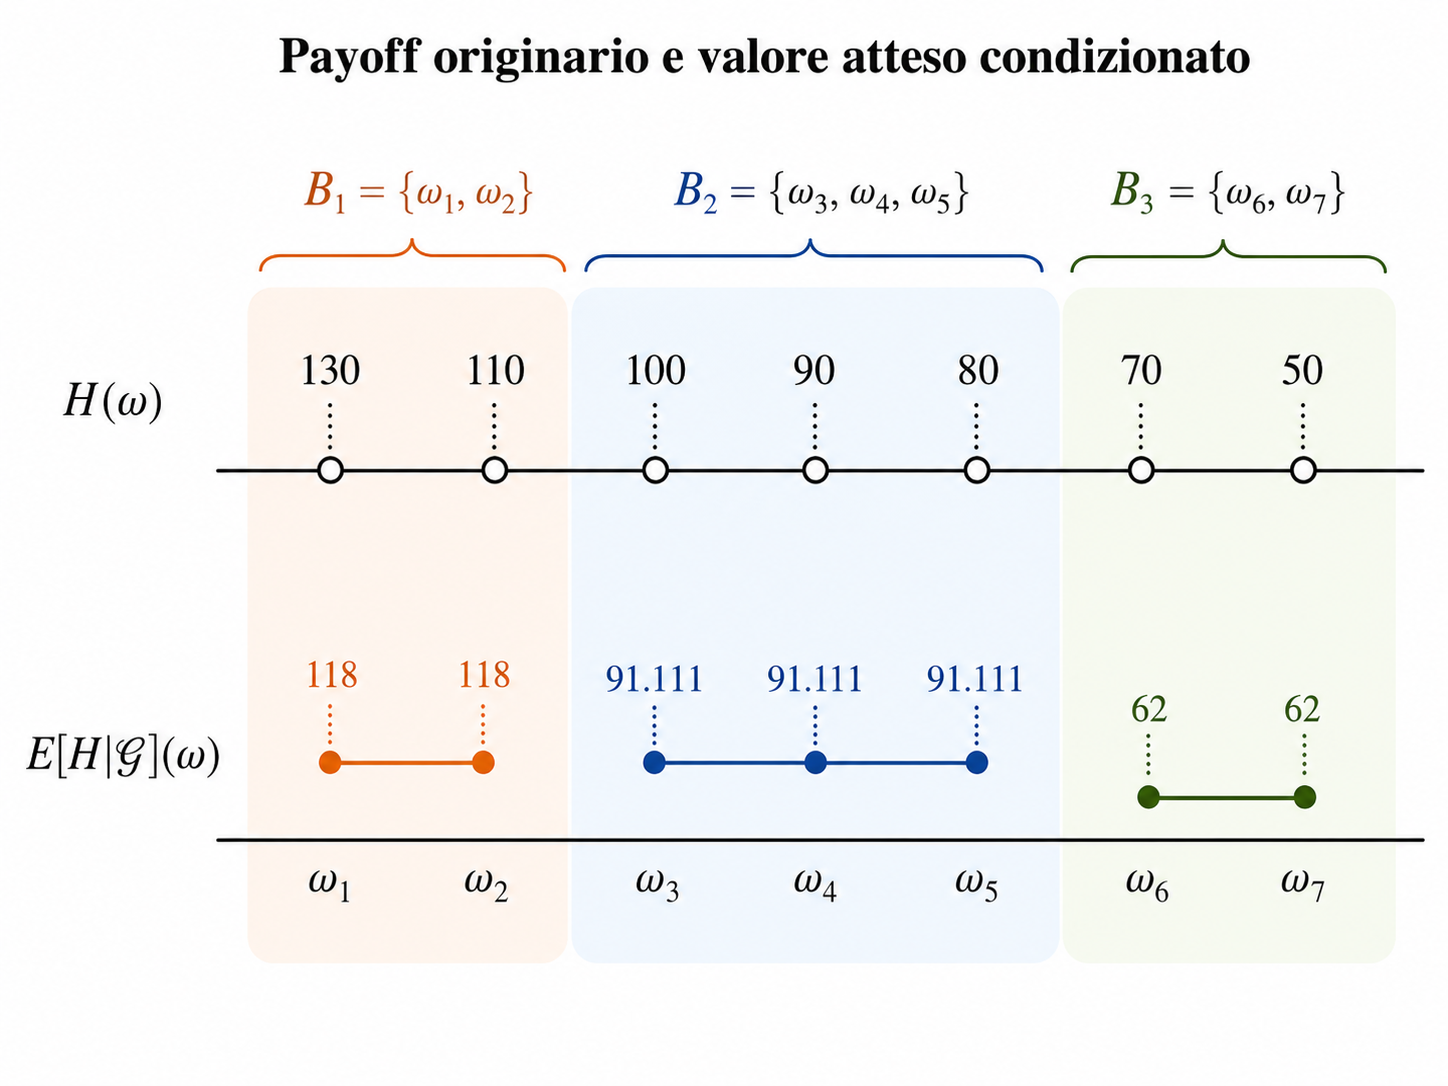
\includegraphics[width=0.88\textwidth,height=0.66\textheight,keepaspectratio]{Cap03_Figura_3_3.png}
\end{center}
\begin{itemize}
\item Il payoff $H$ distingue i sette esiti elementari.
\item La previsione $Z=\E[H\mid\G]$ distingue \textbf{soltanto i tre atomi}.
\end{itemize}

%TCIMACRO{\TeXButton{EndFrame}{\end{frame}}}%
%BeginExpansion
\end{frame}%
%EndExpansion
%*********************************************
\subsection{Informazione fine e grossolana}
%TCIMACRO{\TeXButton{BeginFrame}{\begin{frame}}}%
%BeginExpansion
\begin{frame}%
%EndExpansion
\QTR{frametitle}{Informazione fine e grossolana}
%TCIMACRO{\TeXButton{Transparency}{\setbeamercovered{transparent=20}}}%
%BeginExpansion
\setbeamercovered{transparent=20}%
%EndExpansion

\begin{center}
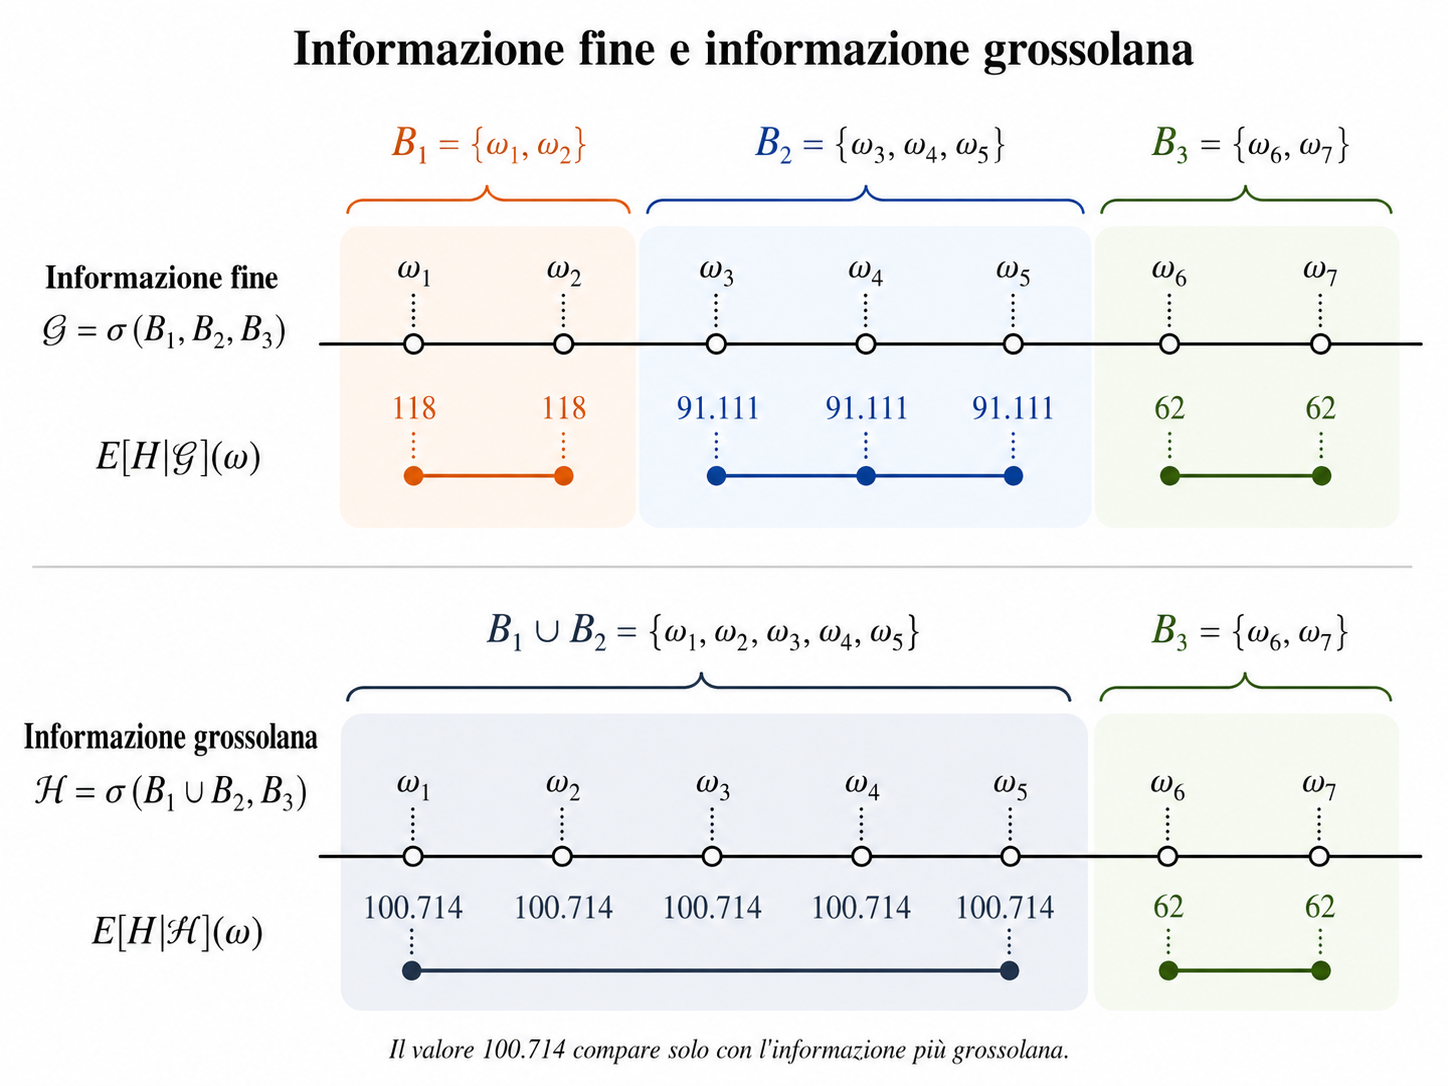
\includegraphics[width=0.84\textwidth,height=0.49\textheight,keepaspectratio]{Cap03_Figura_3_4.png}
\end{center}
\vspace{-1mm}
\[
\mathcal H=\sigma(B_1\cup B_2,B_3)\subseteq\G.
\]
\begin{itemize}
\item Con $\mathcal H$ non distinguiamo pi\`{u} $B_1$ da $B_2$.
\item La previsione sul blocco aggregato diventa
$\E[H\mid B_1\cup B_2]\simeq100.714$.
\end{itemize}

%TCIMACRO{\TeXButton{EndFrame}{\end{frame}}}%
%BeginExpansion
\end{frame}%
%EndExpansion

\section{Dalle partizioni al segnale continuo}
%*********************************************
\subsection{Partizioni progressivamente pi\`{u} fini}
%TCIMACRO{\TeXButton{BeginFrame}{\begin{frame}}}%
%BeginExpansion
\begin{frame}%
%EndExpansion
\QTR{frametitle}{Partizioni progressivamente pi\`{u} fini}
%TCIMACRO{\TeXButton{Transparency}{\setbeamercovered{transparent=20}}}%
%BeginExpansion
\setbeamercovered{transparent=20}%
%EndExpansion

\textbf{Problema.} Un segnale di mercato $S$ pu\`{o} assumere un continuo di valori.
\medskip
\textbf{Strategia.} Prima di osservare il valore esatto, distinguiamo
soltanto la \textbf{classe} in cui cade $S$.
\medskip
\begin{center}
\begin{tabular}{c|c|c}
Informazione & Classi informative & Previsione \\
\hline
$\G_1$ & 2 intervalli & $Z_1=\E[X\mid\G_1]$ \\
$\G_2$ & 4 intervalli & $Z_2=\E[X\mid\G_2]$ \\
$\G_3$ & 8 intervalli & $Z_3=\E[X\mid\G_3]$ \\
$\vdots$ & $\vdots$ & $\vdots$
\end{tabular}
\end{center}
\medskip
\[
\G_1\subseteq\G_2\subseteq\G_3\subseteq\cdots
\]
\begin{center}
\textcolor{light-blue}{Raffinare una partizione significa distinguere pi\`{u} situazioni informative.}
\end{center}

%TCIMACRO{\TeXButton{EndFrame}{\end{frame}}}%
%BeginExpansion
\end{frame}%
%EndExpansion
%*********************************************
\subsection{Il caso continuo come limite delle previsioni}
%TCIMACRO{\TeXButton{BeginFrame}{\begin{frame}}}%
%BeginExpansion
\begin{frame}%
%EndExpansion
\QTR{frametitle}{Il caso continuo come limite delle previsioni}
%TCIMACRO{\TeXButton{Transparency}{\setbeamercovered{transparent=20}}}%
%BeginExpansion
\setbeamercovered{transparent=20}%
%EndExpansion

\textbf{Caso finito.} Per ogni $n$, la previsione $Z_n=\E[X\mid\G_n]$
\`{e} costruita come media sui blocchi di una partizione finita.
\medskip
\textbf{Passaggio al limite.} Scegliamo le partizioni in modo da ottenere,
nel loro insieme, tutta l'informazione generata dal segnale $S$:
\[
\G=\sigma(S)
=\sigma\!\left(\bigcup_{n=1}^{\infty}\G_n\right).
\]
Per $X$ integrabile vale il risultato teorico
\[
\boxed{Z_n=\E[X\mid\G_n]\longrightarrow\E[X\mid\G].}
\]
\begin{itemize}
\item Le previsioni sui blocchi diventano progressivamente pi\`{u} dettagliate.
\item Il limite \`{e} la previsione condizionata all'informazione del segnale continuo.
\end{itemize}
{\scriptsize\textcolor{light-blue}{Il risultato teorico di convergenza (quasi certa e in $L^1$) non viene dimostrato.}}

%TCIMACRO{\TeXButton{EndFrame}{\end{frame}}}%
%BeginExpansion
\end{frame}%
%EndExpansion
%*********************************************
\subsection{La torre: coerenza fra livelli informativi}
%TCIMACRO{\TeXButton{BeginFrame}{\begin{frame}}}%
%BeginExpansion
\begin{frame}%
%EndExpansion
\QTR{frametitle}{La torre: coerenza fra livelli informativi}
%TCIMACRO{\TeXButton{Transparency}{\setbeamercovered{transparent=20}}}%
%BeginExpansion
\setbeamercovered{transparent=20}%
%EndExpansion

\textbf{Ipotesi.} $X$ integrabile e $\mathcal H\subseteq\G$.
\medskip
\textbf{Propriet\`{a} della torre:}
\[
\boxed{\E\bigl[\E[X\mid\G]\mid\mathcal H\bigr]
=\E[X\mid\mathcal H].}
\]
\medskip
\begin{itemize}
\item La previsione con informazione \textbf{fine}, ricalcolata usando
l'informazione \textbf{grossolana}, coincide con la previsione fatta
direttamente con quest'ultima.
\item Scegliendo $\mathcal H=\{\varnothing,\Omega\}$ si recupera
$\E[\E[X\mid\G]]=\E[X]$.
\end{itemize}
\medskip
\begin{center}
\textcolor{light-blue}{Il principio prepara il condizionamento all'informazione disponibile a tempi diversi.}
\end{center}

%TCIMACRO{\TeXButton{EndFrame}{\end{frame}}}%
%BeginExpansion
\end{frame}%
%EndExpansion

\section{Esercizio svolto in aula}
%*********************************************
\subsection{Esercizio: una perdita continua in condizioni di stress}
%TCIMACRO{\TeXButton{BeginFrame}{\begin{frame}}}%
%BeginExpansion
\begin{frame}%
%EndExpansion
\QTR{frametitle}{Esercizio: una perdita continua in condizioni di stress}
%TCIMACRO{\TeXButton{Transparency}{\setbeamercovered{transparent=20}}}%
%BeginExpansion
\setbeamercovered{transparent=20}%
%EndExpansion

\textbf{Dati.} La perdita $L$ di un portafoglio, in milioni di euro,
\`{e} uniformemente distribuita su $[0,20]$:
\[
f_L(\ell)=
\begin{cases}
1/20,&0\leq\ell\leq20,\\
0,&\text{altrimenti}.
\end{cases}
\]
Definiamo l'evento di stress:
\[
A=\{L>15\}.
\]
\textbf{Quesiti da svolgere in aula:}
\begin{enumerate}
\item Calcolare la perdita media $\E[L]$ e la probabilit\`{a} $\Prob(A)$.
\item Ricavare la densit\`{a} condizionata $f_{L\mid A}$.
\item Calcolare $\E[L\mid A]$.
\item Verificare i risultati e interpretarli finanziariamente.
\end{enumerate}

%TCIMACRO{\TeXButton{EndFrame}{\end{frame}}}%
%BeginExpansion
\end{frame}%
%EndExpansion
%*********************************************
\subsection{Soluzione I: perdita media e probabilit\`{a} di stress}
%TCIMACRO{\TeXButton{BeginFrame}{\begin{frame}}}%
%BeginExpansion
\begin{frame}%
%EndExpansion
\QTR{frametitle}{Soluzione I: perdita media e probabilit\`{a} di stress}
%TCIMACRO{\TeXButton{Transparency}{\setbeamercovered{transparent=20}}}%
%BeginExpansion
\setbeamercovered{transparent=20}%
%EndExpansion

\textbf{1. Perdita media prima di osservare lo stress.}
\[
\begin{aligned}
\E[L]&=\int_0^{20}\ell\,f_L(\ell)\,d\ell
=\frac1{20}\int_0^{20}\ell\,d\ell\\
&=\frac1{20}\left[\frac{\ell^2}{2}\right]_0^{20}
=\frac{400}{40}=10.
\end{aligned}
\]
\medskip
\textbf{2. Probabilit\`{a} dell'evento di stress.}
\[
\begin{aligned}
\Prob(A)&=\Prob(L>15)=\int_{15}^{20}\frac1{20}\,d\ell\\
&=\frac{20-15}{20}=\frac14=0.25.
\end{aligned}
\]
\medskip
\begin{center}
\textcolor{light-blue}{La perdita media iniziale \`{e} 10 milioni; la probabilit\`{a} di stress \`{e} il 25\%.}
\end{center}

%TCIMACRO{\TeXButton{EndFrame}{\end{frame}}}%
%BeginExpansion
\end{frame}%
%EndExpansion
%*********************************************
\subsection{Soluzione II: densit\`{a} dopo lo stress}
%TCIMACRO{\TeXButton{BeginFrame}{\begin{frame}}}%
%BeginExpansion
\begin{frame}%
%EndExpansion
\QTR{frametitle}{Soluzione II: densit\`{a} dopo lo stress}
%TCIMACRO{\TeXButton{Transparency}{\setbeamercovered{transparent=20}}}%
%BeginExpansion
\setbeamercovered{transparent=20}%
%EndExpansion

\textbf{3. Distribuzione di $L$ dopo aver osservato $A=\{L>15\}$.}
\medskip
La densit\`{a} condizionata \`{e} nulla fuori da $(15,20]$.
All'interno dell'intervallo \`{e} proporzionale alla densit\`{a} iniziale:
\[
f_{L\mid A}(\ell)=
\begin{cases}
\displaystyle\frac{f_L(\ell)}{\Prob(A)}
=\frac{1/20}{1/4}=\frac15,&15<\ell\leq20,\\[2mm]
0,&\text{altrimenti}.
\end{cases}
\]
\textbf{Controllo della normalizzazione:}
\[
\int_{-\infty}^{+\infty}f_{L\mid A}(\ell)\,d\ell
=\int_{15}^{20}\frac15\,d\ell
=\frac{20-15}{5}=1.
\]
\begin{center}
\textcolor{light-blue}{La perdita resta uniforme, ma il supporto si restringe agli esiti di stress.}
\end{center}

%TCIMACRO{\TeXButton{EndFrame}{\end{frame}}}%
%BeginExpansion
\end{frame}%
%EndExpansion
%*********************************************
\subsection{Soluzione III: valore atteso condizionato allo stress}
%TCIMACRO{\TeXButton{BeginFrame}{\begin{frame}}}%
%BeginExpansion
\begin{frame}%
%EndExpansion
\QTR{frametitle}{Soluzione III: valore atteso condizionato allo stress}
%TCIMACRO{\TeXButton{Transparency}{\setbeamercovered{transparent=20}}}%
%BeginExpansion
\setbeamercovered{transparent=20}%
%EndExpansion

\textbf{4. Calcolo della perdita attesa sapendo che $L>15$.}
\[
\begin{aligned}
\E[L\mid A]
&=\int_{15}^{20}\ell\,f_{L\mid A}(\ell)\,d\ell
=\frac15\int_{15}^{20}\ell\,d\ell\\
&=\frac15\left[\frac{\ell^2}{2}\right]_{15}^{20}
=\frac{400-225}{10}=17.5.
\end{aligned}
\]
\medskip
\textbf{Verifica con la formula dell'indicatrice.}
\[
\begin{aligned}
\E[L\1_A]&=\int_{15}^{20}\frac{\ell}{20}\,d\ell
=\frac{400-225}{40}=4.375,\\
\E[L\mid A]&=\frac{\E[L\1_A]}{\Prob(A)}
=\frac{4.375}{0.25}=17.5.
\end{aligned}
\]
\begin{center}
\textcolor{light-blue}{L'informazione di stress porta la perdita attesa da 10 a 17.5 milioni.}
\end{center}

%TCIMACRO{\TeXButton{EndFrame}{\end{frame}}}%
%BeginExpansion
\end{frame}%
%EndExpansion
%*********************************************
\subsection{Soluzione IV: coerenza e interpretazione finanziaria}
%TCIMACRO{\TeXButton{BeginFrame}{\begin{frame}}}%
%BeginExpansion
\begin{frame}%
%EndExpansion
\QTR{frametitle}{Soluzione IV: coerenza e interpretazione finanziaria}
%TCIMACRO{\TeXButton{Transparency}{\setbeamercovered{transparent=20}}}%
%BeginExpansion
\setbeamercovered{transparent=20}%
%EndExpansion

\textbf{5. Verifica mediante valore atteso totale.}
\medskip
Fuori dallo stress, $A^c=\{L\leq15\}$ e la perdita \`{e}
uniforme su $[0,15]$:
\[
\E[L\mid A^c]=\frac{0+15}{2}=7.5,
\qquad \Prob(A^c)=0.75.
\]
Quindi:
\[
\begin{aligned}
\E[L]
&=\E[L\mid A]\Prob(A)
 +\E[L\mid A^c]\Prob(A^c)\\
&=17.5\cdot0.25+7.5\cdot0.75\\
&=4.375+5.625=10.
\end{aligned}
\]
\textbf{Interpretazione.} La condizione di stress aumenta la perdita
media prevista del 75\% rispetto alla media ex ante; non altera i possibili
valori di $L$, ma modifica quali valori sono compatibili con l'informazione.

%TCIMACRO{\TeXButton{EndFrame}{\end{frame}}}%
%BeginExpansion
\end{frame}%
%EndExpansion

\section{Sintesi}
%*********************************************
\subsection{Sintesi: dalla media all'informazione nel tempo}
%TCIMACRO{\TeXButton{BeginFrame}{\begin{frame}}}%
%BeginExpansion
\begin{frame}%
%EndExpansion
\QTR{frametitle}{Sintesi: dalla media all'informazione nel tempo}
%TCIMACRO{\TeXButton{Transparency}{\setbeamercovered{transparent=20}}}%
%BeginExpansion
\setbeamercovered{transparent=20}%
%EndExpansion

\begin{center}
\begin{tabular}{c|l}
Oggetto & Informazione utilizzata \\
\hline
$\E[X]$ & Nessuna informazione aggiuntiva \\
$\E[X\mid A]$ & Un evento $A$: si ottiene un numero \\
$\E[X\mid\G]$ & Una sigma-algebra: si ottiene una variabile casuale
\end{tabular}
\end{center}
\medskip
\begin{itemize}
\item Partizioni finite: la previsione \`{e} costante su ciascun atomo.
\item Un segnale continuo pu\`{o} essere avvicinato tramite partizioni
progressivamente pi\`{u} fini.
\item La \textbf{torre} garantisce coerenza fra diversi livelli informativi.
\end{itemize}
\medskip
\begin{center}
\textcolor{light-blue}{Nella Lezione 5: $\F_0\subseteq\F_1\subseteq\cdots\subseteq\F_T$ descrive l'informazione che cresce nel tempo.}
\end{center}

%TCIMACRO{\TeXButton{EndFrame}{\end{frame}}}%
%BeginExpansion
\end{frame}%
%EndExpansion

\end{document}
